%% example.tex
%% Jeremy Singer
%% 16 Oct 12

\documentclass{mpaper}

\usepackage[caption=false]{subfig}

\begin{document}

\title{QUICsilver: Optimising QUIC for use with Real-Time Multimedia Traffic}
\author{Vivian Band}
\matricnum{2038561}

\maketitle

\begin{abstract}
  % Four sentences:
  %  - State the problem
  The vast majority of IP traffic (~80\%) is multimedia traffic. Teleconferencing and online gaming are commonly used applications on the modern Internet; these need to appear to respond in real-time to user input and require low latency to achieve this.
  
  QUIC is seeing more adoption as a transport protocol for client-server applications, accounting for a signficant portion of Google's outbound traffic and making up ~7\% of total Internet traffic as of 2017. However, it is not currently suitable for real-time traffic due to high latency caused by guaranteed reliability and in-order delivery.
  
  %  - Say why it's an interesting problem
  QUIC is a userspace protocol; these can be modified more easily than kernel-level implementations of transport protocols, like TCP. This flexibility allows QUIC to be significantly adapted, allowing the protocol to be used for real-time multimedia applications.
  
  %  - Say what your solution achieves
  The modifications made in this project allow QUIC to achieve low-latency by allowing some packet loss, subject to playback deadlines, in order to improve the throughput of data to the receiver application. Video playback quality is further improved by taking advantage of existing retransmission behaviours in QUIC, allowing the retransmission of frames which will still be useful when they reach the receiver as well as any dependent frames required for live ones.
  
  %  - Say what follows from your solution
  Our solution shows that partial reliability through the use of deadline-aware retransmissions minimises the occurrence of stalls by improving the throughput of useful ('live') multimedia data. This use of selective retransmissions is particularly important in loss-prone environments (e.g. wireless links).
  

\end{abstract}

%==================================================================================================
\section{Introduction}

% A good paper introduction is fairly formulaic. If you follow a simple set
% of rules, you can write a very good introduction. The following outline can
% be varied. For example, you can use two paragraphs instead of one, or you
% can place more emphasis on one aspect of the intro than another. But in all
% cases, all of the points below need to be covered in an introduction, and
% in most papers, you don't need to cover anything more in an introduction.
%
% Paragraph 1: Motivation. At a high level, what is the problem area you
% are working in and why is it important? It is important to set the larger
% context here. Why is the problem of interest and importance to the larger
% community?



% Paragraph 2: What is the specific problem considered in this paper? This
% paragraph narrows down the topic area of the paper. In the first
% paragraph you have established general context and importance. Here you
% establish specific context and background.



% Paragraph 3: "In this paper, we show that...". This is the key paragraph
% in the introduction - you summarize, in one paragraph, what are the main
% contributions of your paper, given the context established in paragraphs 
% 1 and 2. What's the general approach taken? Why are the specific results
% significant? The story is not what you did, but rather:
%  - what you show, new ideas, new insights
%  - why interesting, important?
% State your contributions: these drive the entire paper.  Contributions
% should be refutable claims, not vague generic statements.

In this paper, we ...

% Paragraph 4: What are the differences between your work, and what others
% have done? Keep this at a high level, as you can refer to future sections
% where specific details and differences will be given, but it is important
% for the reader to know what is new about this work compared to other work
% in the area.



% Paragraph 5: "We structure the remainder of this paper as follows." Give
% the reader a road-map for the rest of the paper. Try to avoid redundant
% phrasing, "In Section 2, In section 3, ..., In Section 4, ... ", etc.

We structure the remainder of this paper as follows.

%==================================================================================================
% Concentrate single-mindedly on a narrative that:
%  - Describes the problem, and why it's interesting
%  - Describes your idea
%  - Defends your idea, showing how it solves the problem, and filling out
%    the details
% On the way, cite relevant work in passing, but defer discussion to the
% end.
%
% Introduce the problem, and your idea, using examples, and only then
% present the general case. Explain the idea as if your were speaking to
% someone using a whiteboard. Conveying the intuition is primary; details
% follow. Write in a top down manner: state broad themes and ideas first,
% then go into details.
%
% The introduction makes claims. The body of the paper provides evidence
% to support each claim. Check each claim in the introduction, identify
% the evidence, and forward-reference it from the claim. 
%==================================================================================================
\section{Background}

% The problem

\subsection{Motivation}

\subsection{Related Work}


%==================================================================================================
\section{Design}

% My idea



%==================================================================================================
\section{Results}

Each test was performed using a simulated network on mininet, consisting of a server node connected to a client node over a single link with a specifically defined latency. This link latency was varied between 50ms, 100ms, and 150ms, and loss rates of 0\%, 0.01\%, 0.1\%, and 1\% were introduced for tests on each latency. Each test ran for 300 seconds with client and server both operating at a framerate of 60 fps; an I-frame was sent every 10th frame, consisting of 4 QUIC packets to represent the fact that I-frames are too large to be sent as a single QUIC payload.

Tests for guaranteed reliability used the \texttt{ngtcp2} QUIC stack with standard retransmission behaviours, while tests for partial reliability used the QUICsilver implementation with selective retransmission mechanisms described above [TODO: write design section].

\subsection{Differences in Stack Latency}

Stack latencies remain consistently within 15ms of the path latency in the partially reliable implementation for all loss rates (figure \ref{stack-par}), but have slightly more variance than stack latencies in the guaranteed reliability implementation in equivalent conditions. This is due to the extra checks which are performed by the server after sending a packet: each item in the retransmission buffer for the relevant stream is checked to see if it has become stale and needs to be removed.

When loss is introduced on the link, the guaranteed reliability implementation begins to show an increase in the number of higher stack latencies \ref{stack-rel}. QUIC determines a packet is lost when it receives an acknowledgement for a higher packet number; this requires a minimum of the time taken to send the packet over the link, plus a multiple of the total round trip time depending on how many times the packet in question was lost in transit. This causes the latency data to gather in bands: the latencies of lost packets will be multiples of the total round-trip time on the link. In contrast, the partially reliable implementation maintains similar performance all rates of loss; this is due to the server removing packets which will not be useful to the client upon arrival from its retransmit buffer without receiving an acknowledgement.

\subsection{Differences in Application Latency}

Partially reliable QUIC achieves consistently lower application latencies for all link latencies compared to standard QUIC with guaranteed reliability (figure \ref{app-par}). Application latencies for partially reliable QUIC have a greater range than stack latencies due to the frame buffer: if there is a gap in received packets, the stack will wait for the missing packet; if the packet doesn't arrive before its predicted playback deadline expires, the read offsets for the stream are advanced and a sequence of video frames with contiguous RTP timestamps is passed to the application (this may only be a single frame). This buffer was intended to be set as 4 frames, corresponding to an additional latency of 66ms at a 60fps playback rate, but was incorrectly set at a single frame during the 50ms and 100ms tests. A single frame at 60fps is equivalent to 16.7ms; this is added to application latency in the event of loss, with decreasing latencies following as subsequent blocks of received frames are passed to the application. In the case of 150ms tests, the buffer limit was set to the intended 4 frames; application latencies can be seen in bands at multiples of 16.7ms to around a maximum of 66.6ms greater than the link latency as a result.

The distinctive four-band pattern present in all instances of partially reliable QUIC is due to I-frames being sent as 4 QUIC packets without a 16.7ms delay between them; four packets must be delivered to the application within the same call, but iterating through the reorder buffer and removing relevant items takes time to execute.

The bands in the guaranteed reliability application latencies are caused by video frames being sent by the server at 16.7ms intervals; the latency of each frame is increased by a multiple of this until the missing packet is received at the client, even though all of these frames are delivered to the application within the same function call. The occasional spikes in 1\% loss test are caused by a packet being lost twice; these occur at twice the round-trip time, plus two frame playback times at 60fps, beyond the initial link latency.

This head-of-line blocking behaviour associated with guaranteed reliability does not affect 0\% loss links, where standard QUIC achieves consistently lower application latencies than partially reliable QUIC, and has minimal impact on average application latency in 0.01\% loss links. However, for 0.1\% and 1\% loss scenarios, partially reliable QUIC achieves consistently lower application latencies: the latencies for fully reliable QUIC in these circumstances are frequently a round-trip time higher than the link latency, compared to a maximum of 66.6ms when a 4-frame buffer is set.

\clearpage

\begin{figure}
 \centering
 \subfloat[Partial reliability, 50ms]{
   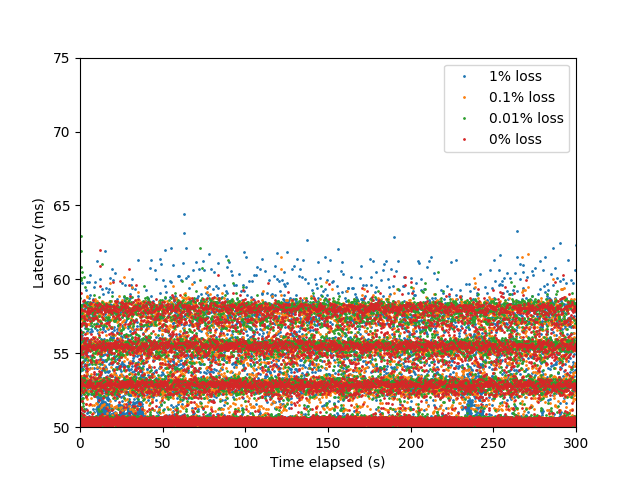
\includegraphics[scale=0.5]{images/graphics-partial/50ms-stack-latencies-combined-PARTIAL.png}
   \label{stack-par-50}
 }
 \\
 \subfloat[Partial reliability, 100ms]{
   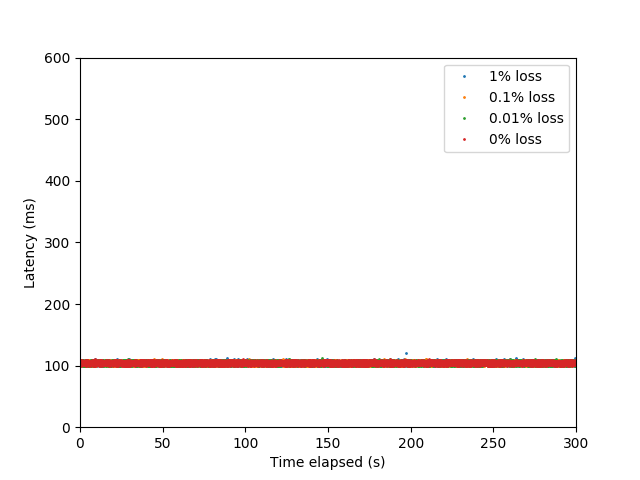
\includegraphics[scale=0.5]{images/graphics-partial/100ms-stack-latencies-combined-PARTIAL.png}
   \label{stack-par-100}
 }
 \\
 \centering
 \subfloat[Partial reliability, 150ms]{
   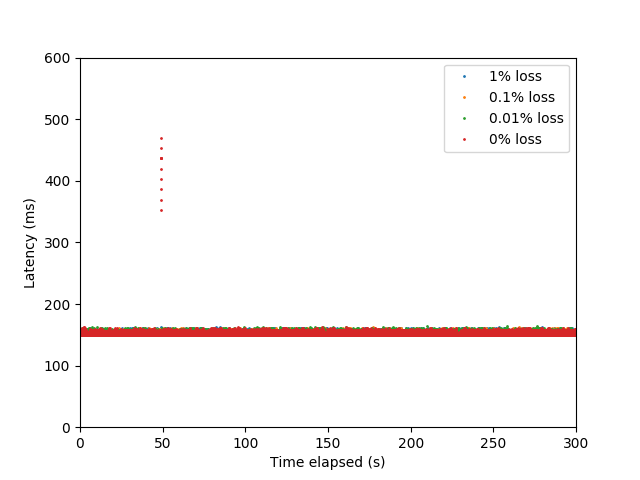
\includegraphics[scale=0.5]{images/graphics-partial/150ms-stack-latencies-combined-PARTIAL.png}
   \label{stack-par-150}
 }
 \caption{Latency between server and client stack (partial reliability)}
 \label{stack-par}
\end{figure}

\begin{figure}
 \centering
 \subfloat[Guaranteed reliability, 50ms]{
   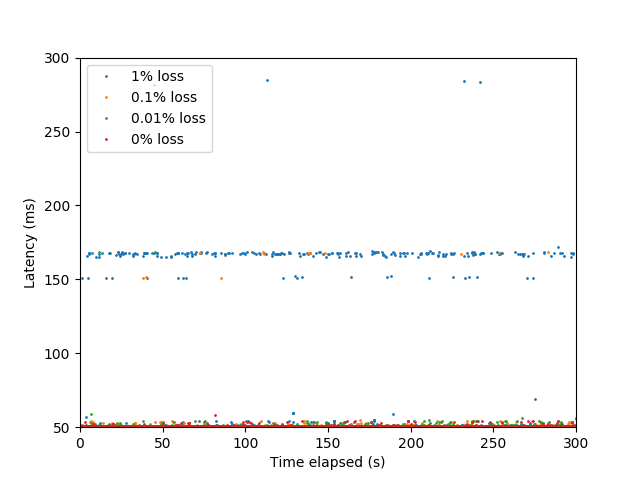
\includegraphics[scale=0.5]{images/graphics-reliable/50ms-stack-latencies-combined-reliable.png}
   \label{stack-rel-50}
 }
 \\
 \subfloat[Guaranteed reliability, 100ms]{
   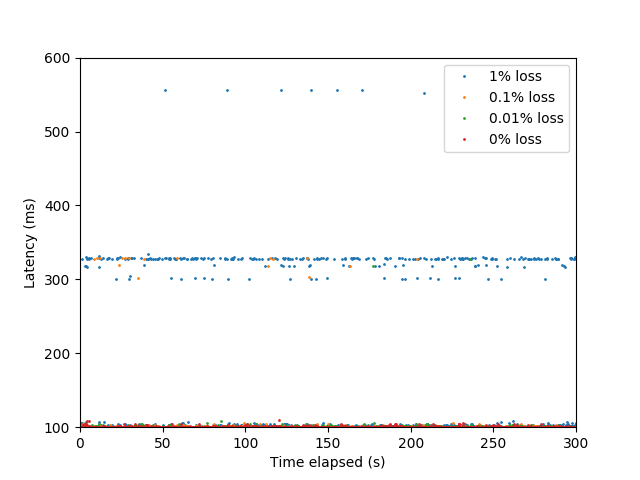
\includegraphics[scale=0.5]{images/graphics-reliable/100ms-stack-latencies-combined-reliable.png}
   \label{stack-rel-100}
 }
 \\
 \centering
 \subfloat[Guaranteed reliability, 150ms]{
   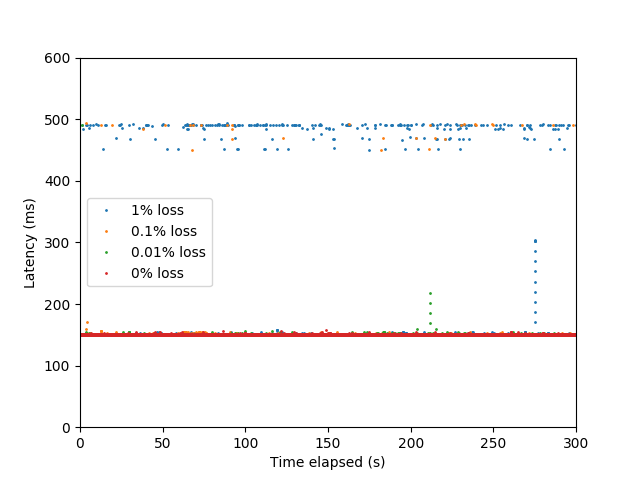
\includegraphics[scale=0.5]{images/graphics-reliable/150ms-stack-latencies-combined-reliable.png}
   \label{stack-rel-150}
 }
 \caption{Latency between server and client stack (guaranteed reliability)}
 \label{stack-rel}
\end{figure}

\clearpage


\begin{figure}
 \centering
 \subfloat[Partial reliability, 50ms]{
   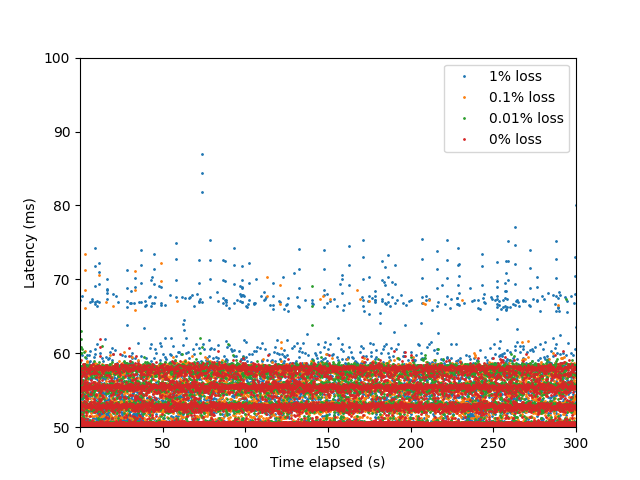
\includegraphics[scale=0.5]{images/graphics-partial/50ms-app-latencies-combined-PARTIAL.png}
   \label{app-par-50}
 }
 \\
 \subfloat[Partial reliability, 100ms]{
   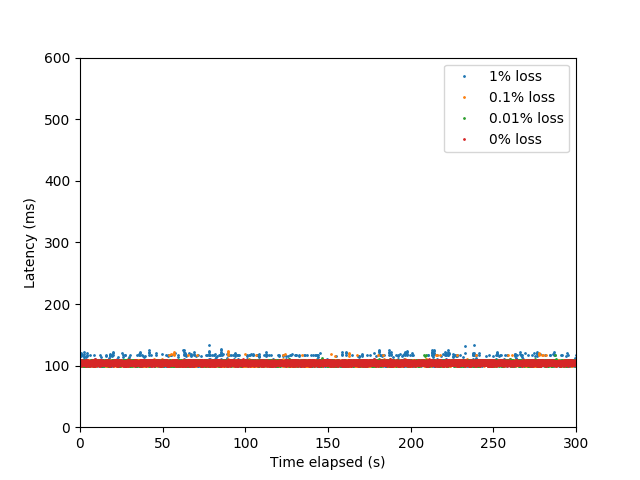
\includegraphics[scale=0.5]{images/graphics-partial/100ms-app-latencies-combined-PARTIAL.png}
   \label{app-par-100}
 }
 \\
 \centering
 \subfloat[Partial reliability, 150ms]{
   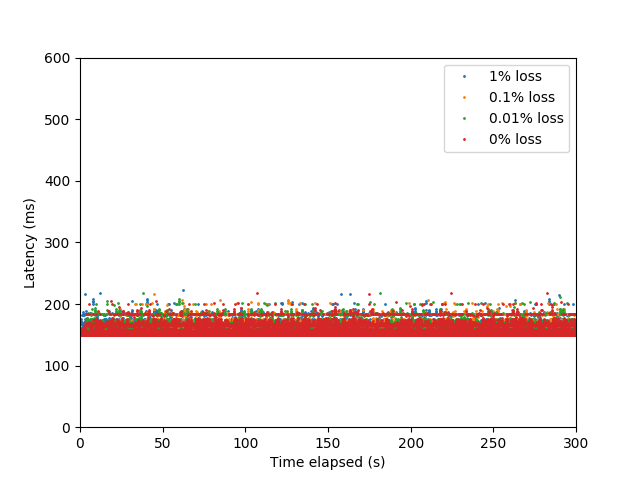
\includegraphics[scale=0.5]{images/graphics-partial/150ms-app-latencies-combined-PARTIAL.png}
   \label{app-par-150}
 }
 \caption{Latency between server and client application (partial reliability)}
 \label{app-par}
\end{figure}

\begin{figure}
 \centering
 \subfloat[Guaranteed reliability, 50ms]{
   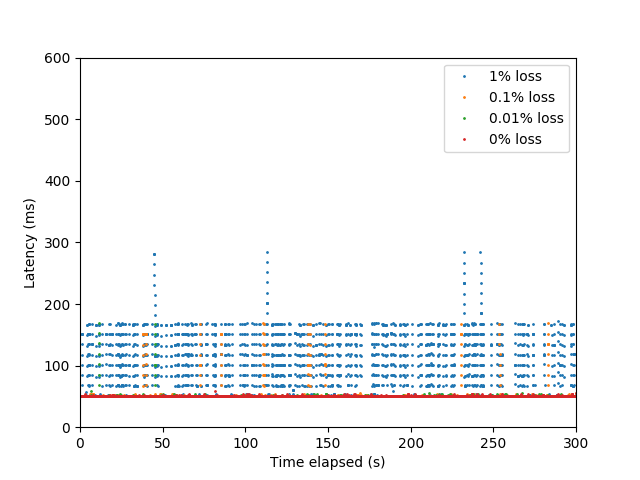
\includegraphics[scale=0.5]{images/graphics-reliable/50ms-app-latencies-combined-reliable.png}
   \label{app-rel-50}
 }
 \\
 \subfloat[Guaranteed reliability, 100ms]{
   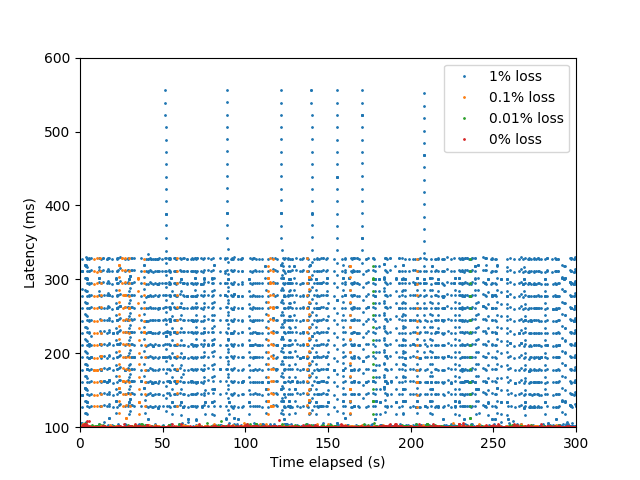
\includegraphics[scale=0.5]{images/graphics-reliable/100ms-app-latencies-combined-reliable.png}
   \label{app-rel-100}
 }
 \\
 \centering
 \subfloat[Guaranteed reliability, 150ms]{
   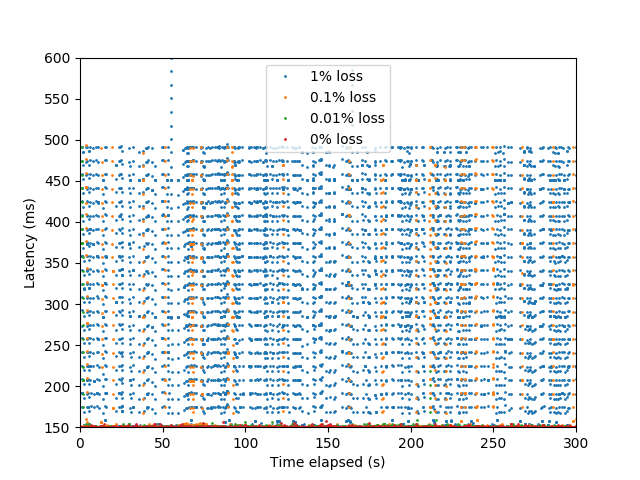
\includegraphics[scale=0.5]{images/graphics-reliable/150ms-app-latencies-combined-reliable.png}
   \label{app-rel-150}
 }
 \caption{Latency between server and client application (guaranteed reliability)}
 \label{app-rel}
\end{figure}




% The details

% Describe results carefully:
%  - clearly state assumptions
%  - give enough information to allow the reader to recreate the results
%  - ensure results are representative; statistically meaningful, etc.
%  - don't overstate results
%  - equally, don't understate them: consider the broader implications


\clearpage
\subsection{Differences in Playback Time}

If a packet has been lost in transit, the head-of-line blocking behaviours within standard QUIC will delay delivering all subsequent data until this missing packet has been received. If there is no video data held in the application to play during this delay (i.e. buffered data), the video will appear to stall. The exact delay caused by a packet lost once is proportional to the path latency: figure \ref{single-50} shows a delay of 100ms, the round trip time of a 50ms link. Figure {single-100} shows a delay of 216ms on a 100ms link, equivalent to a round trip time plus one frame playback time; this extra 16ms is likely due to these measurements being obtained in terms of RTP playback timestamps, with a granularity of 16ms per increment at 60fps. The delay for a loss on a 150ms link shown in figure \ref{single-150} is 333ms, equivalent to one round-trip time plus one frame playback time.

\begin{figure}
 \centering
 \subfloat[Single instance playback delay, 50ms]{
   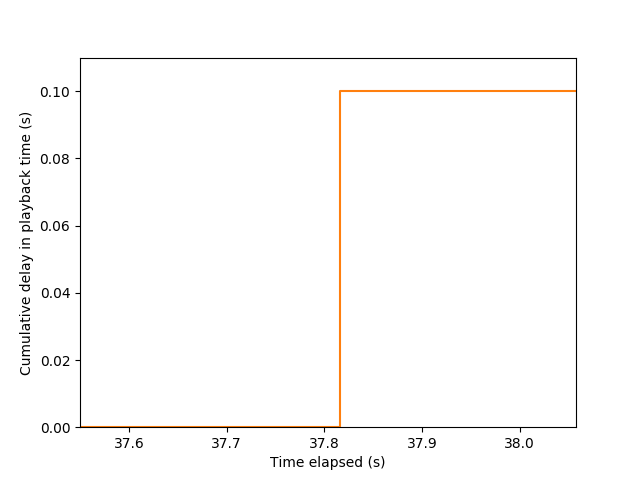
\includegraphics[scale=0.5]{images/offsets-single.png}
   \label{single-50}
 }
 \\
 \subfloat[Single instance playback delay, 100ms]{
   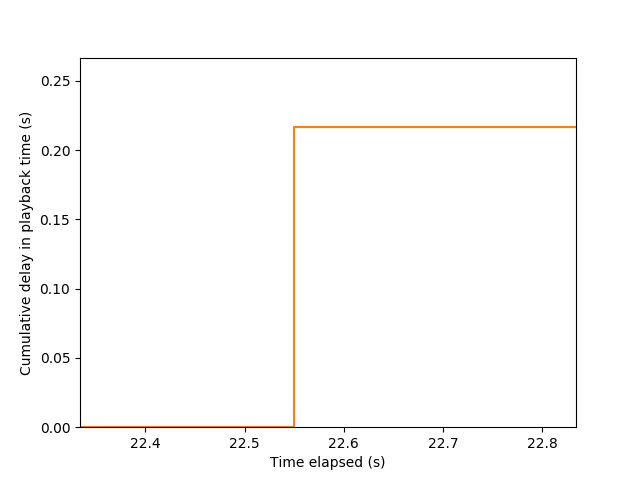
\includegraphics[scale=0.5]{images/offsets-single-100ms.png}
   \label{single-100}
 }
 \\
 \centering
 \subfloat[Single instance playback delay, 150ms]{
   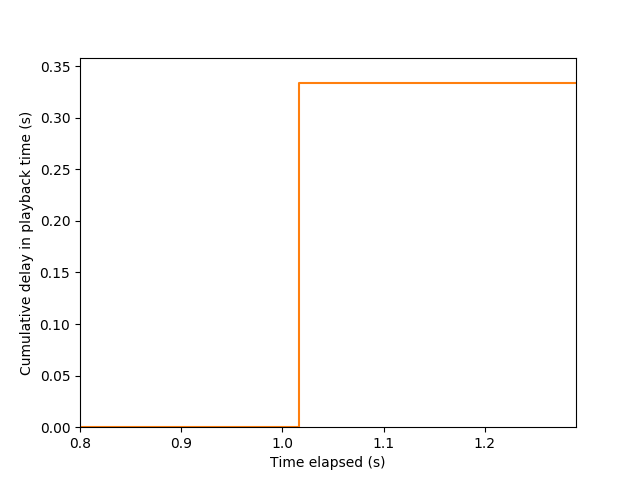
\includegraphics[scale=0.5]{images/offsets-single-150ms.png}
   \label{single-150}
 }
 \caption{Increase in cumulative playback delay as a result of a single lost packet on various links (guaranteed reliability)}
 \label{single-rel}
\end{figure}

As the rate of loss on a link increases, the number of stalls also increases. Table \ref{reliable-stalls} shows the number of stalls which occured in the 100ms tests; naturally, the number of stalls between all latencies remain similar for each loss rate, but the difference between intended playback time and actual playback time for each subsequent video frame becomes larger at higher latencies (table \ref{relative-offset-table}). The graphs shown in figure \ref{playback-rel} illustrate the magnitude of these differences.

\begin{table}[h!]
\centering
\label{stalls-data-rel}
\begin{center}
%\begin{tabular}{|p{5cm}|l|p{8.5cm}|}
\begin{tabular}{|p{2cm}|p{2cm}|p{2cm}|}
\hline
Loss Rate & Stalls & Frames Played\\ \hline
0\% & 0 & 100.0\% \\ \hline
0.01\%  & 2 & 100.0\% \\ \hline
0.1\%  & 12 & 100.0\% \\ \hline
1\%  & 198 & 100.0\% \\ \hline

\end{tabular}
\caption{Number of stalls and percentage of frames played for guaranteed reliability, 100ms}
\label{reliable-stalls}
\end{center}
\end{table}

\begin{figure}
 \centering
 \subfloat[Playback offsets, 50ms]{
   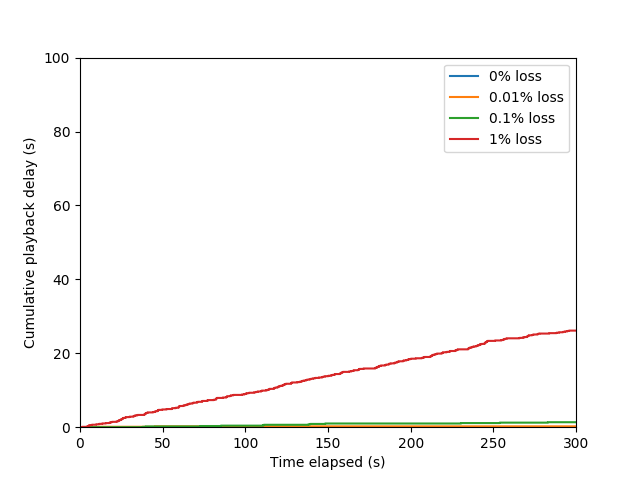
\includegraphics[scale=0.5]{images/graphics-reliable/50ms-offsets-combined-reliable.png}
   \label{playback-rel-50}
 }
 \\
 \subfloat[Playback offsets, 100ms]{
   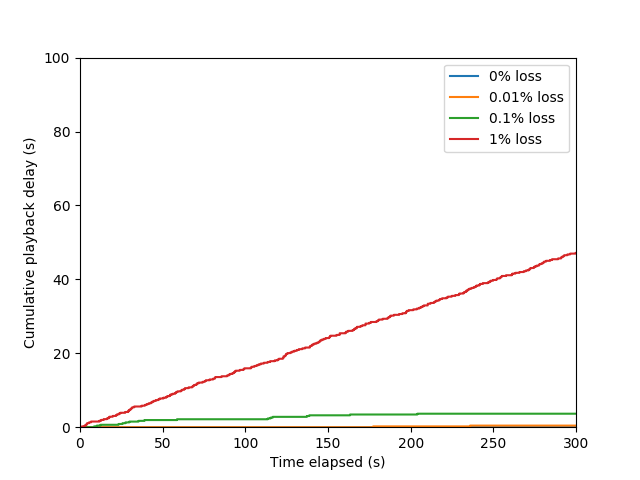
\includegraphics[scale=0.5]{images/graphics-reliable/100ms-offsets-combined-reliable.png}
   \label{playback-rel-100}
 }
 \\
 \centering
 \subfloat[Playback offsets, 150ms]{
   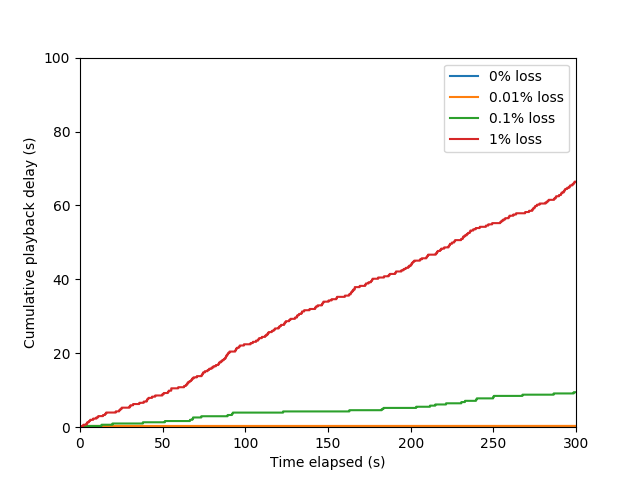
\includegraphics[scale=0.5]{images/graphics-reliable/150ms-offsets-combined-reliable.png}
   \label{playback-rel-150}
 }
 \caption{Differences between when a frame is played out compared to the intended playback time (guaranteed reliability)}
 \label{playback-rel}
\end{figure}

\begin{figure}
 \centering
 \subfloat[Playback times, 50ms]{
   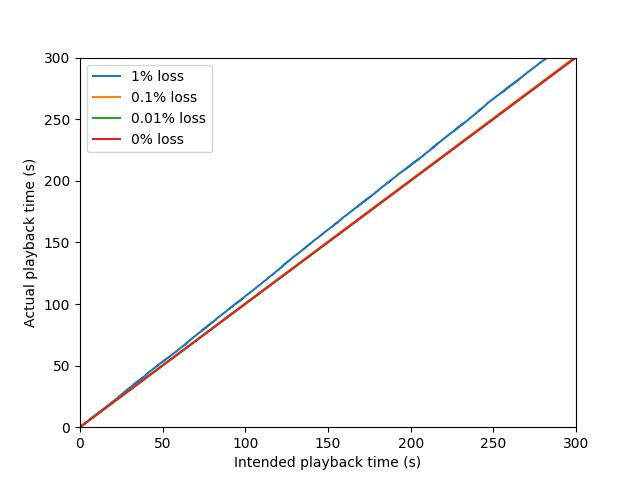
\includegraphics[scale=0.5]{images/graphics-reliable/50ms-relative-offsets-combined-reliable.png}
   \label{playback-offsets-rel-50}
 }
 \\
 \subfloat[Playback times, 100ms]{
   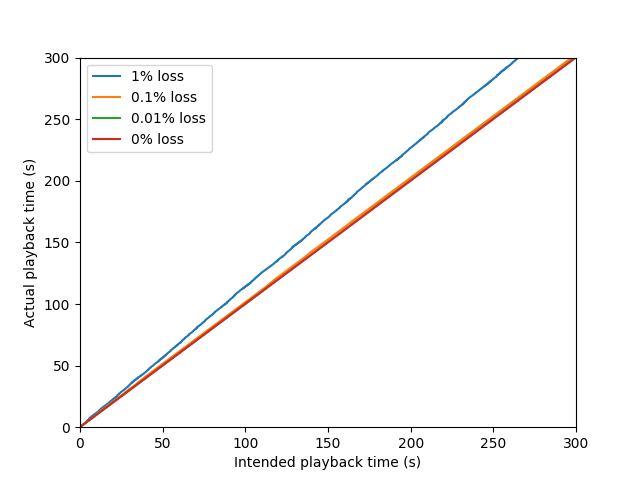
\includegraphics[scale=0.5]{images/graphics-reliable/100ms-relative-offsets-combined-reliable.png}
   \label{playback-offsets-rel-100}
 }
 \\
 \centering
 \subfloat[Playback times, 150ms]{
   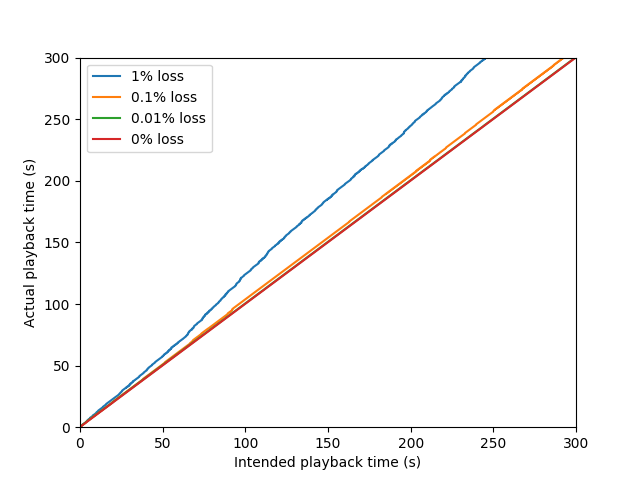
\includegraphics[scale=0.5]{images/graphics-reliable/150ms-relative-offsets-combined-reliable.png}
   \label{playback-offsets-rel-150}
 }
 \caption{Differences between when a frame is played out compared to when the frame was sent (guaranteed reliability)}
 \label{playback-offsets-rel}
\end{figure}

\begin{table}[h!]
\centering
\label{stalls-data-rel}
\begin{center}
%\begin{tabular}{|p{5cm}|l|p{8.5cm}|}
\begin{tabular}{|p{1.5cm}|p{1.5cm}|p{2cm}|p{2cm}|}
\hline
Loss Rate & Latency (ms) & Discrepancy (s) & Total latency (s)\\ \hline
0.01\%  & 50 & 0.2 & 50.2 \\ \hline
0.1\%  & 50 & 1.2 & 51.2 \\ \hline
1\%  & 50 & 19.8 & 69.8 \\ \hline
0.01\%  & 100 & 0.43 & 100.43 \\ \hline
0.1\%  & 100 & 2.6 & 102.6 \\ \hline
1\%  & 100 & 42.8 & 142.8 \\ \hline
0.01\%  & 150 & 0.66 & 150.66 \\ \hline
0.1\%  & 150 & 4.0 & 154.0 \\ \hline
1\%  & 150 & 66.0 & 216.0 \\ \hline

\end{tabular}
\caption{Playback discrepancy and total latency for a live-recorded frame to be played by the client application at the end of each test run for each loss rate and latency for guaranteed reliability}
\label{relative-offset-table}
\end{center}
\end{table}

Table \ref{relative-offset-table} shows the cumulative discrepancy between intended playback time and actual playback time, as well as the delay between a live-recorded frame being sent and being played by the client application by the end of a 300 second test run. The increase in this delay over time is illustrated in figure \ref{playback-offsets-rel}.

Although 100\% of the video frames in the media content being sent are delivered to the client application with guaranteed reliability behaviours, there is an increasing latency between sending a frame and playing it at the client; the longer an application is running, the greater this playback discrepancy becomes. The path latencies in these tests were constant, but path latencies `in the wild' are variable, and occasionally subject to spikes if a link is congested. The total playback discrepancy suffered by an application would sharply increase as a result of these spikes; a return to lower latencies afterwards would not reduce it.

It should also be noted that this discrepancy is applied to packets which have not been lost in transit: lost packets are subject to even higher latencies, and are increased by multiples of the round-trip time depending on the number of times they are lost. As shown in figure \ref{app-rel}, packets which have been received before a missing packet but have a higher packet number also suffer from increased application latency. International Telecommunication Recommendation G.114 recommends no more than 150ms latency ``mouth-to-ear'' for audio communications \cite{ITU-REC}; the path latency must be even smaller than this to allow for time to capture live audio and video and to perform codec processing. Figure \ref{app-rel} shows that fully reliable QUIC stays within this limit at 0\% and 0.01\% loss for 50ms and 100ms links, but it often exceeds even the ``mouth-to-ear'' limit at 0.1\% and 1\% loss for all links; 0\% and 0.01\% loss flows on a 150ms link cannot satisfy the recommended latency requirement due to the link latency. Gaming has even stricter latency bounds [TODO: I know gaming latencies should be around 80ms or below anecdotally, but need a citation with exact bounds for this].

In the case of video streaming, content buffering can be used to disguise stalls. For example, if a user wanted to stream a 1 hour, pre-recorded video, the client might buffer a given amount of content before starting playback. Given that an I-frame is sent every 10th frame as 4 QUIC packets, 216,000 video frames will be sent using 280,800 QUIC packets in total: 28 stalls can be expected to occur at 0.01\% loss, 281 stalls at 0.1\% loss, and 2808 stalls at 1\% loss. At a cumulative latency increase of 100ms per lost packet on a 50ms link, a buffer of 200 seconds should completely conceal stalls for 0.01\% and 0.1\% loss rates, and will conceal stalls at 1\% until 2564 seconds (around 43 minutes) into playback. For a 100ms link with a 216ms latency increase, a buffer of 200 seconds should completely conceal stalls for 0.01\% and 0.1\% loss rates, and will conceal stalls until 1183 seconds (around 20 minutes) into playback. A 400 second buffer should conceal all stalls. However, buffering is not a feasible strategy for reducing the number of stalls in real-time media delivery: live-generated content cannot be buffered in advance, and buffering does not reduce the cumulative playback delay created as a result of stalls in fully reliable QUIC.


%\begin{figure}
% \centering
% \subfloat[Playback times, 50ms]{
%   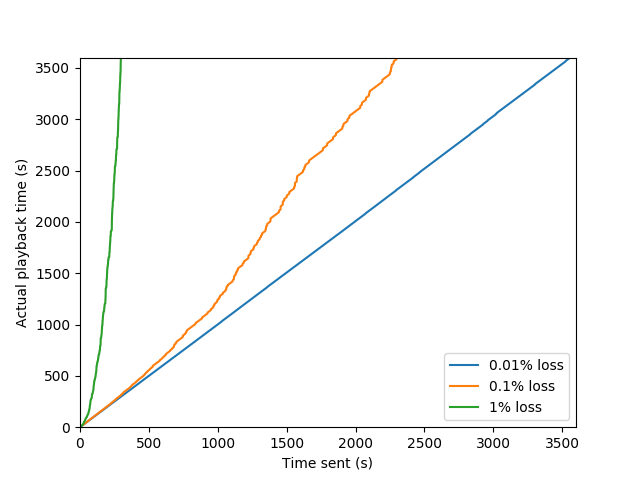
\includegraphics[scale=0.5]{images/graphics-1hr/50ms-1hr-relative-offsets-combined-reliable.png}
%   \label{stall-concealment-50}
% }
% \\
% \subfloat[Playback times, 100ms]{
%   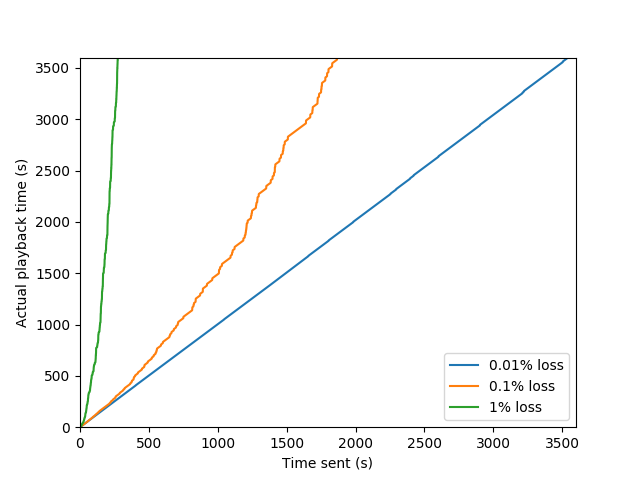
\includegraphics[scale=0.5]{images/graphics-1hr/100ms-1hr-relative-offsets-combined-reliable.png}
%   \label{stall-concealment-100}
% }
% \caption{Cumulative playback delay charted against buffered video data (guaranteed reliability)}
% \label{stall-concealment}
%\end{figure}

The partially reliable implementation of QUIC created for this project experiences no stalls due to incrementing stream read offsets in response to playback deadlines: if there is a gap in the data received on a given stream and there is data approaching its playback deadline held in the reorder buffer, the modified implementation will skip ahead to the live data and will not wait for the preceding gap to be filled. This allows the client to play received content without additional delays caused by head-of-line blocking. The percentage of `useful frames' in table \ref{par-playback-stats} is calculated as the number of complete I-frames and P-frames with an associated complete I-frame, compared to the total number of unique frames sent by the server; incomplete I-frames and their subsequent P-frames are not useful for playback.

\begin{table}[h!]
\centering
\label{stalls-data-par}
\begin{center}
%\begin{tabular}{|p{5cm}|l|p{8.5cm}|}
\begin{tabular}{|p{2cm}|p{2cm}|p{2cm}|}
\hline
Loss Rate & Stalls & Useful frames\\ \hline
0\% & 0 & 100.0\% \\ \hline
0.01\%  & 0 & 100.0\% \\ \hline
0.1\%  & 0 & 99.644\% \\ \hline
1\%  & 0 & 95.472\% \\ \hline

\end{tabular}
\caption{Number of stalls and percentage of useful frames played for partial reliability}
\label{par-playback-stats}
\end{center}
\end{table}

\begin{figure}[h]
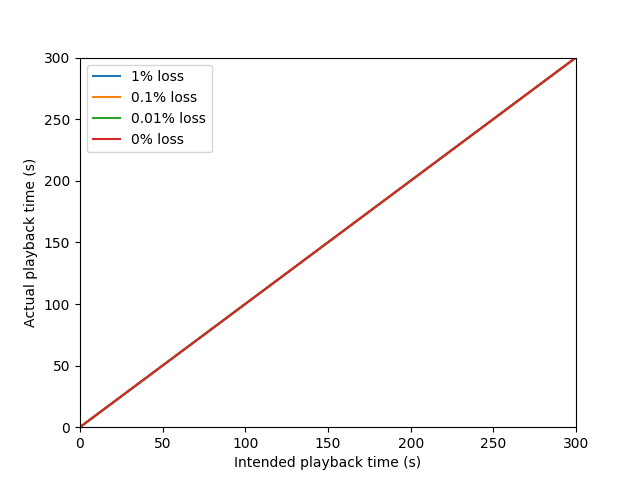
\includegraphics[scale=0.5]{images/graphics-partial/50ms-relative-offsets-combined-PARTIAL.png}
\centering
\caption{Differences between when a frame is played out compared to when the frame was sent (partial reliability, all loss rates)}
\label{playback-par}
\end{figure}

Fewer frames are played back at the client, which will result in occasional glitches in playback. Given that 1 in every 10 frames sent is an I-frame consisting of 4 QUIC packets, there is a 70\% chance that a dropped packet contains a P-frame; at a playback rate of 60fps, this would result in an absence of updated content for 16.7ms. If a dropped packet contains a section of an I-frame, this will affect the subsequent 9 P-frames which are dependent on it; this would result in no the appearance of glitched content for 167ms due to P-frames acting in reference to an incorrect I-frame.

As described in section 3, the partially reliable implementation of QUIC is capable of performing retransmissions of live I-frames and P-frames, and stale I-frames which are still required for live P-frames. A 4-frame delay adds a maximum of 66.6ms additional latency between the server and the client application, which would create a total maximum of 116.6ms on a 50ms link; this is already relatively high for a real-time application. Removing this delay entirely results in the implementation achieving the lowest possible latency while effectively transmitting P-frames unreliably and retransmitting I-frames once at most.

Whether a stale I-frame can be retransmitted to enable the playback of future P-frames depends on the path latency: if an I-frame is sent once every 10 frames, there is a a space of 150ms between I-frames being played back. Given that a retransmission takes one round-trip time in total, an I-frame fragment would enable the 9th subsequent P-frame if it was sent over a 66.6ms latency link; lower latencies would allow a larger number of associated P-frames to be played successfully, while any latency above this would not perform any retransmissions. Sending I-frames less frequently would allow a larger window for I-frame fragments to be retransmitted, but the amount of glitched playback would increase in proportion with the link latency; the longer an application has to wait for a complete I-frame, the more P-frames are played in reference to the incorrect I-frame.

For a test run of 300 seconds, 18,000 video frames are sent. On average 180 of these are dropped in the worst-case 1\% loss scenario; if 30\% of these are I-frames and 70\% are P-frames, 11.01 seconds of playback in total are subject to glitches across all latencies. This is higher than the total playback offset in a 50ms connection subject to 1\% loss for guaranteed reliability (table \ref{relative-offset-table}), but the crucial difference between these two outcomes is that the content received after a loss in the partially reliable implementation is played without any cumulative delay (figure \ref{playback-par}): some playback quality is sacrificed for maintaining a consistent low latency to allow for the level of responsiveness required by real-time applications.

An application using guaranteed reliability could discard stale frames and continue playback from the frame with the closest RTP timestamp to the current playback deadline to reduce this cumulative delay, but it would play fewer frames than the partially reliable implementation: the minimum and maximum absences of correctly updated content for partially reliable QUIC for all link latencies are 16.7ms and 167ms respectively, while delays in the datasets gathered for fully reliable QUIC range between 100ms and 333ms, depending on the link latency. This shows that partially reliable QUIC results in improved throughput of useful data compared to attempting to optimise applications on top of standard QUIC for real-time behaviour.

\clearpage
%==================================================================================================
\section{Related Work}

% This should come near the end, and focussing on discussing how your work
% relates to that of others. Any relevant related work should have been
% cited already, so this is not a list of related work, it's a discussion
% of how that work relates.
%
% Why not put related work after the introduction? 1) because describing
% alternative approaches gets between the reader and your idea; and 2)
% because the reader knows nothing about the problem yet, so your
% (carefully trimmed) description of various technical trade-offs is
% absolutely incomprehensible.
% 
% When writing the related work:
%  - Give credit to others where it's due; this doesn't diminish the
%    credit you get from your paper. 
%  - Acknowledge weaknesses in your approach.
%  - Ensure related work is accurate and up-to-date



%==================================================================================================
%==================================================================================================
\section{Future Work}

\subsection{Congestion Control}
Removing an item from the retransmission buffer in the \texttt{ngtcp2} implementation of QUIC is complex. The function call used to receive an acknowledgement contains numerous updates to congestion control statistics; simply attempting to remove the item from the retransmit buffer by freeing the associated memory causes a range of errors due to failed \texttt{assert} checks elsewhere in the stack. As a result, falsified acknowledgements were created at the server to remove stale entries which had not received an acknowledgement from the client. This is problematic in that it causes the client to believe there is no congestion on the network, and this QUIC flow becomes overly aggressive compared to other flows sharing the link as a result. This did not cause problems with testing on the simple one-to-one topology with a known round-trip time and no co-existing flows described in section 4, but the congestion control statistics must be more carefully adjusted in future iterations to allow real-time QUIC flows to be fair to other traffic on shared links.


\subsection{Improved I-frame Handling}
QUIC packets containing fragments of I-frames which will not arrive in time to be played back themselves, but are required for live P-frames are retransmitted by the server. An implementation of real-time QUIC which immediately passes data to the application upon arrival would deliver these `stale' fragments to the application, however, the implementation of partial reliability which delivers video frames in order does not; the stream read offsets at the client are incremented upon the delivery of live data and the detection of stale data, so these I-frame fragments are never passed to the application.

Future refinements of this implementation would include mechanisms to allow the client to determine if an incoming packet contains an I-frame based on its associated RTP timestamp, and introducing additional read offsets within a stream to allow required stale I-frames to be read without also reading stale P-frame data in the process. This would allow complete frames to be delivered in-order to the application, while continuing to drop stale P-frames and stale I-frames with no live dependencies to minimise latency. I-frame payloads would also need to be read as a complete block to allow delivery to the application as a complete frame, as opposed to the current method of being delivered as several separate reads.

\subsection{Multiple Streams}
Real-time QUIC will allow multimedia application developers to use multiplexed streams to deliver data to an application concurrently, but this significantly increases the difficulty in developing these applications: the content received from each stream needs to be co-ordinated in order to be used by the application correctly. The tests in this paper were performed using a single stream; further experiments will focus on how to co-ordinate multiplexed streams to optimise the quality of video playback.

%==================================================================================================
\section{Conclusions}

\subsection{Placement of Complexity}
Passing QUIC payloads (i.e. RTP packets) to the application as soon as they arrive avoids adding even more complexity to an already extensive transport protocol, but it requires application developers to implement mechanisms to reorder incoming frames, assemble I-frames, and deal with frames which are corrupted, incomplete, or missing dependencies; the transport protocol effectively becomes RTP with selective retransmissions. This allows developers flexibility in exactly how a given application should behave while improving the amount of useful data received, but it increases both the entry barrier to creating real-time multimedia applications and the difficulty in maintaining them.

Delivering complete video frames in-order while allowing gaps, as the implementation of real-time QUIC in this project aims to do, removes the responsibility of frame reordering and reconstruction from application developers, but increases the complexity of QUIC while also restricting the applications which can be developed: novel applications, such as multiplayer gaming over QUIC, may require many different types of messages other than I-frames and P-frames. Awareness of these messages would need to be added within the QUIC protocol in order for a receiver to be able to parse stream information as a complete message, and for the sender to be able to establish more complex dependencies and retransmission behaviours; for example, an important message such as a character receiving an item should be transmitted with guaranteed reliability and only removed from the retransmission buffer with a client-sent ACK, while movement would use partial reliability and deadline-based removal in a similar manner to P-frames. This is simply not feasible given the wide range of behaviours and transmittable information that real-time applications could have.

\subsection{Partial Reliability for Other Real-Time Applcations}
The development of video-based real-time applications which rely on a limited number of message types (I-frames and P-frames) can be simplified by making QUIC aware of how to parse these messages and pass them to the application as complete frames in sequential order; this project has been successful in achieving improved real-time video playback performance using this approach. However, the increasing popularity of real-time applications with variable information and behaviour, such as augmented reality, virtual reality, and multiplayer gaming, suggests that passing data to the application as soon as it arrives is the better approach to take for a generalised real-time implementation of QUIC. This prevents ossification in terms of which applications which can use real-time QUIC and also avoids adding an unrealistic level of complexity to QUIC implementations. Creating a new partially reliable QUIC stream type for use alongside guaranteed reliability streams would ensure that key information reaches the receiver while allowing low-latency for other content.


\subsection{Uses for Partially Reliable QUIC}
QUICsilver is 

%more accurate measuring of useful frames if data delivered in-order to application as complete frame - incomplete I-frame would still pose problems even if data was immediately passed to application from stack



\end{document}
